\documentclass{article}

\usepackage[utf8]{vietnam}
\usepackage{multirow}
\usepackage{graphicx}
\usepackage{setspace}
\usepackage{fancyhdr}
\usepackage{pifont}

\usepackage{tikz}
\usetikzlibrary{calc}

\usepackage[left=3.5cm,right=2cm,top=2cm,bottom=2cm]{geometry}

\usepackage{listings}
\usepackage{color}

\definecolor{dkgreen}{rgb}{0,0.6,0}
\definecolor{gray}{rgb}{0.5,0.5,0.5}
\definecolor{mauve}{rgb}{0.58,0,0.82}

\lstset{frame=tb,
  language=Java,
  aboveskip=3mm,
  belowskip=3mm,
  showstringspaces=false,
  columns=flexible,
  basicstyle={\big\ttfamily},
  numbers=left,
  numberstyle=\small\color{gray},
  keywordstyle=\color{blue},
  commentstyle=\color{dkgreen},
  stringstyle=\color{mauve},
  breaklines=true,
  breakatwhitespace=true,
  tabsize=3
}

\usepackage[none]{hyphenat}
\tolerance=9999
\emergencystretch=10pt
\hyphenpenalty=10000
\exhyphenpenalty=100

\newcommand\para{\paragraph{} \hspace{0pt} \fontsize{13}{13}\selectfont \fontseries{b}\selectfont \indent}
\newcommand\subpara{\fontsize{13}{13}\selectfont \fontseries{b}\selectfont}
\newcommand\head{\fontsize{30}{20}\selectfont \fontseries{b}\selectfont}

\makeatletter
\renewcommand{\tableofcontents}{%
	\@starttoc{toc}%
}
\makeatother

\begin{document}
    \begin{tikzpicture}[overlay,remember picture]
    \draw [line width=2pt]
        ($ (current page.north west) + (3.0cm,-2.0cm) $)
        rectangle
        ($ (current page.south east) + (-2.0cm,2.5cm) $);
    \draw [line width=0.5pt]
        ($ (current page.north west) + (3.1cm,-2.1cm) $)
        rectangle
        ($ (current page.south east) + (-2.1cm,2.6cm) $);
    \end{tikzpicture}

	\begin{center}
		\pagenumbering{gobble}
		\fontsize{14}{20}\selectfont
		\textbf{ĐẠI HỌC QUỐC GIA HÀ NỘI\\
			\textbf{TRƯỜNG ĐẠI HỌC KHOA HỌC TỰ NHIÊN\\}
			\textbf{KHOA TOÁN - CƠ - TIN HỌC}}
		\vspace{0.8cm}
		\begin{figure}[htp]
			\begin{center}
				
\includegraphics[scale=0.5]{logohus.png}
			\end{center}
		\end{figure}
		\fontsize{16}{20}\selectfont\textbf{BÁO CÁO CUỐI KỲ\\}
		\fontsize{20}{20}\selectfont\textbf{CÁC THÀNH PHẦN PHẦN MỀM\\}
	\vspace{1cm}
		\setstretch{1.5}
	    \fontsize{18}{18}\selectfont\textbf{Tên Đề Tài: DESIGN PATTERNS}
\textit{(nhóm 1)\\}
	    \vspace{1cm}
	 \end{center}

    \begin{flushleft}
		\fontsize{16}{20}\selectfont
		\textit{Sinh viên thực hiện:}\\
		\textbf{Phạm Bá Thắng - 20001976}\\
		\textbf{La Thị Anh Thư - 20001980}\\
    \end{flushleft}
	\vspace{3cm}
    \begin{center}
		\fontsize{14}{20}\selectfont
		\textbf{HÀ NỘI, 1/2022}
	\end{center}
	\pagebreak

	\pagestyle{fancy}
	\fancyhf{}
	\chead{\thepage}
	\renewcommand{\headrulewidth}{0pt}
	\begin{center}
		\head{LỜI CẢM ƠN}
		\hspace{15pt}
	\end{center}
	    \para{Đầu tiên, chúng em xin gửi lời cảm ơn chân thành đến Trường Đại học Khoa học Tự nhiên đã đưa môn học Các thành phần phần mềm vào chương trình giảng dạy. Đặc biệt, chúng em xin gửi lời cảm ơn sâu sắc đến giảng viên bộ môn - Thầy Quản Thái Hà đã dạy dỗ, truyền đạt những kiến thức quý báu cho chúng em trong suốt thời gian học tập vừa qua. Trong thời gian tham gia lớp học Các thành phần phần mềm của thầy, chúng em đã có thêm cho mình nhiều kiến thức bổ ích, tinh thần học tập hiệu quả, nghiêm túc. Đây chắc chắn sẽ là hành trang để chúng em có thể vững bước sau này.}
	    \para{Bộ môn Các thành phần phần mềm là môn học thú vị, vô cùng bổ ích và có tính thực tế cao. Đảm bảo cung cấp đủ kiến thức, gắn liền với nhu cầu phát triển của sinh viên. Tuy nhiên, khả năng tiếp nhận kiến thức của mỗi người luôn tồn tại những hạn chế nhất định. Do đó, bài báo cáo khó có thể tránh khỏi những thiếu sót. Kính mong thầy xem xét và góp ý để bài báo cáo của chúng em được hoàn thiện hơn.}
	    \para{Kính chúc thầy sức khỏe, hạnh phúc, thành công trên con đường sự nghiệp giảng dạy.}
	\pagebreak


	\begin{center}
		\head{Mục Lục}
	\end{center}
	\setstretch{1.5}
	\fontsize{13}{13}\selectfont
	\tableofcontents
\pagebreak


	\pagenumbering{arabic}\setcounter{page}{1}
	\begin{center}
		\fontsize{30}{20}\selectfont \part{Tóm tắt}
	\end{center}
	    \para{Design pattern là các giải pháp tổng thể đã được tối ưu hóa, được tái sử dụng cho các vấn đề phổ biến trong thiết kế phần mềm mà chúng ta thường gặp phải hàng ngày. Đây là tập các giải pháp đã được suy nghĩ, đã giải quyết trong tình huống cụ thể.}
	    \para{Design patterns có thể thực hiện được ở phần lớn các ngôn ngữ lập trình. Nó giúp bạn giải quyết vấn đề một cách tối ưu nhất, cung cấp cho bạn các giải pháp trong lập trình hướng đối tượng (OOP).}
	    \para{Design parttern gồm 23 loại được chia thành 3 nhóm:}

	    \begin{itemize}
	        \item[-]\subpara{Creational Pattern (nhóm khởi tạo) gồm: Factory Method, Abstract Factory, Builder, Prototype, Singleton. Những Design pattern loại này cung cấp một giải pháp để tạo ra các object và che giấu được logic của việc tạo ra nó, thay vì tạo ra object một cách trực tiếp bằng cách sử dụng method new. Điều này giúp cho chương trình trở nên mềm dẻo hơn trong việc quyết định object nào cần được tạo ra trong những tình huống được đưa ra}
	        \item[-]\subpara{Structural Pattern (nhóm cấu trúc) gồm: Adapter, Bridge, Composite, Decorator, Facade, Flyweight và Proxy. Những Design pattern loại này liên quan tới class và các thành phần của object. Nó dùng để thiết lập, định nghĩa quan hệ giữa các đối tượng.}
	        \item[-]\subpara{Behavioral Pattern (nhóm hành vi) gồm: Interpreter, Template Method, Chain of Responsibility, Command, Iterator, Mediator, Memento, Observer, State, Strategy và Visitor. Nhóm này dùng trong thực hiện các hành vi của đối tượng, sự giao tiếp giữa các object với nhau.}
	    \end{itemize}
    \pagebreak
		\begin{center}
		\fontsize{30}{20}\selectfont\part{Nhóm Khởi tạo - Creational Pattern}
	    \end{center}
	\pagebreak

		\section{Singleton}
        \subsection{Định Nghĩa Và Mô Hình Cấu Trúc}
        \begin{itemize}
            \item[-]\subpara{Singleton đảm bảo chỉ duy nhất một instance được tạo ra và cung cấp một method để có thể truy xuất được instance đó mọi lúc mọi nơi trong chương trình.}
            \item[-]\subpara{Singleton ẩn đi hàm dựng của class và sử dụng hàm các hàm có sẵn bên trong để tạo đối tượng}
        \end{itemize}
		\begin{figure}[htp]
			\begin{center}
				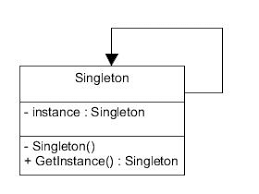
\includegraphics[scale=1]{singleton-pattern.png}
			\end{center}
		\end{figure}

        \subsection{Đặc điểm}
        \begin{itemize}
            \item[-]\subpara{Đảm bảo rằng một lớp chỉ có một instance}
            \item[-]\subpara{Dễ dàng truy cập vào instance này}
            \item[-]\subpara{Kiểm soát việc khởi tạo nó}
            \item[-]\subpara{Giới hạn số lượng instance}
            \item[-]\subpara{Có thể truy cập như một biến toàn cục}
        \end{itemize}
		\subsection{Mục Đích Sử Dụng}
		\begin{itemize}
			\item[-]\subpara{Là dạng class nên có thể sử dụng với nhiều design parttern khác nhau}
			\item[-]\subpara{Sử dụng làm biến toàn cục với các ưu điểm như:}
			\begin{itemize}
			    \item[+]\subpara{Không làm rối loạn danh sách các biến toàn cục vì không tạo ra các biến không cần thiết}
			    \item[+]\subpara{Chúng cho phép phân bổ và khởi tạo khi cần (call-by-need), trong khi tạo nhiều các biến toàn cục ngay từ đầu sẽ luôn tiêu tốn tài nguyên.}
		    \end{itemize}
		    \item[-]\subpara{Ví dụ như dùng để ghi log rất thích hợp vì chúng ta chỉ cần 1 bản ghi log duy nhất cho mỗi phiên đồng thời lại cần ở tất cả cácbộ phân của chương trình}
		\end{itemize}

		\subsection{Code khuôn mẫu}
		\begin{lstlisting}
    public class Singleton {
        private static final Singleton INSTANCE = new Singleton();
        private Singleton() {}
        public static Singleton getInstance(){
            if(instance == null){
                instance = new Singleton();
            }
            return instance;
        }
    }
        \end{lstlisting}

		\subsection{Giải thích Design Pattern}
		\begin{itemize}
			\item[-]\subpara{Private constructor để hạn chế truy cập từ class bên ngoài.}
			\item[-]\subpara{Đặt private static final variable đảm bảo biến chỉ được khởi tạo trong class và duy nhất 1 lần.}
			\item[-]\subpara{Có một method public static để return instance được khởi tạo ở trên và một đoạn if để kiểm tra xem instance tồn tại chưa, nếu chưa sẽ gọi hàm khởi tạo. Hàm này được gọi là accessor.}
			\item[-]\subpara{Sau đó là các hàm để sử dụng.}
		\end{itemize}

		\subsection{Ví Dụ Sử Dụng Trong Thực Tế}
            \subpara{Simple Logger\\https://github.com/blaplafla13th/design-partterns/tree/main/src/singleton}
    \para{Tạo một logger theo Singleton parttern, sau đó chúng ta thêm các hàm kiểm tra file (check), hàm ghi file (write) và hàm đọc file (read). Khi runtime, các Exception được ghi lại và chuyển sang String rồi ghi ra file, sau đó file được đọc. Khi dùng trong package, người dùng có thể gọi 3 hàm read write và chỉ cần gọi đối tượng mà không cần khởi tạo lại đối tượng Log.}
		\pagebreak

		\section{Builder}
        \subsection{Định Nghĩa Và Mô Hình Cấu Trúc}
        \begin{itemize}
            \item[-]\subpara{}<ý 1>
            \item[-]\subpara{}<ý 2>
        \end{itemize}

        \subsection{Đặc điểm}
        \begin{itemize}
            \item[-]\subpara{}<đặc điểm 1>
            \item[-]\subpara{}<đặc điểm 2>
        \end{itemize}

		\subsection{Mục Đích Sử Dụng}
		\begin{itemize}
			\item[-]\subpara{}<mục đích 1>
			\item[-]\subpara{}<mục đích 2>
		\end{itemize}


		\subsection{Code khuôn mẫu}
		\begin{lstlisting}
package builder.pattern;
//Builder.java
public interface Builder {
    public void buildPartOne();
    public void buildPartTwo();
    public Product getProduct();
}

//Client.java
public class Client {
    public static void main(String[] args) {
        Director director = new Director(new ConcreteBuilder());
        director.makeProduct();

        Product product = director.getProduct();

        System.out.println("Product part: " + product.getPartOne());
        System.out.println("Product part: " + product.getPartTwo());
    }
}

//ConcreteBuilder.java
public class ConcreteBuilder implements Builder{
    private Product product;

    public ConcreteBuilder() {
        this.product = new Product();
    }

    @Override
    public void buildPartOne() {
        product.setPartOne("Part One");
    }

    @Override
    public void buildPartTwo() {
        product.setPartTwo("Part Two");
    }

    @Override
    public Product getProduct() {
        return product;
    }
}

//Director.java
public class Director {
    private Builder builder;

    public Director(Builder builder){
        this.builder = builder;
    }

    public void makeProduct(){
        builder.buildPartOne();
        builder.buildPartTwo();
    }

    public Product getProduct(){
        return builder.getProduct();
    }
}

//Product.java
public class Product {
    private String partOne;
    private String partTwo;

    public String getPartOne() {
        return partOne;
    }

    public void setPartOne(String partOne) {
        this.partOne = partOne;
    }

    public String getPartTwo() {
        return partTwo;
    }

    public void setPartTwo(String partTwo) {
        this.partTwo = partTwo;
    }
}
        \end{lstlisting}

		\subsection{Giải thích Design Pattern}
		\begin{itemize}
			\item[-]\subpara{Product: đại diện cho đối tượng cần tạo, đối tượng này phức tạp, có nhiều thuộc tính.}
			\item[-]\subpara{Builder: là abstract class hoặc interface khai báo phương thức tạo đối tượng.}
			\item[-]\subpara{ConcreteBuilder: kế thừa Builder và cài đặt chi tiết cách tạo ra đối tượng. Nó sẽ xác định và nắm giữ các instance mà nó tạo ra, đồng thời nó cũng cung cấp phương thức để trả các các thể hiện mà nó đã tạo ra trước đó. Hay nói cách khác là bản thiết kế từng bước của đối tượng Product}
			\item[-]\subpara{Director/Client: là nơi sẽ gọi tới Builder để tạo ra đối tượng.}
			\item[-]\subpara{Khi chạy main của Client, đối tượng Director được khởi tạo, với đối đầu vào là 1 instance ConcreteBuilder được kế thừa từ Builder chứa thông tin từng bước}
			\item[-]\subpara{Tiếp theo Client gọi hàm thực thi trong Director là hàm chạy chứa các bước trong interface builder từ đó gọi các hàm override bởi các hàm trong Builder ConcreteBuilder để thực hiện các bước dựng đối tượng}
			\item[-]\subpara{Sau khi Director dựng xong đối tượng, Client lấy đối tượng Product về từ Director từ đó có thể sử dụng Product như bình thường}
		\end{itemize}

		\subsection{Ví Dụ Sử Dụng Trong Thực Tế}
\begin{itemize}
            \item[-]\subpara{Hệ thống quản lý tài khoản sử dụng builder parttern\\ https://github.com/blaplafla13th/design-partterns/tree/main/src/builder}
            \item[-]\subpara{Do tạo tài khoản hay đăng nhập, chúng ta cùng có hai bước là ghi nhận thông tin và xử lý thông tin như vậy chúng ta cần tạo một interface AccountBuilder với 2 step để xử lý với step 1 là điền thông tin, step 2 là xử lý dữ liệu và đọc ghi vào mảng cụ thể là accountArrayList ở Client.java. Tiếp theo tạo class builder của signIn và signUp để tạo form điền ở step1 và xử lý form ở step2.}
            \item[-]\subpara{Chúng ta tạo một AccountDirector để tạo đối tượng builder để chạy hai builder vừa tạo. Hàm dựng sẽ nhận bản thiết kế của class builder và thực hiện các bước. sau đó là hàm để return đối tượng}
            \item[-]\subpara{Về phía Client, ta cần tạo 1 arraylist để lưu tại khoản và hàm để gọi arraylist này. Trong main ta tạo biến current để lưu tài khoản hiện tại đóng vai trò quản lý phiên. Tạo một vòng lặp để lựa chọn đăng kí và đăng nhập và 2 director tương ứng với 2 lựa chọn đăng kí và đăng nhập. Tiếp theo chúng ta sẽ chạy hàm sign của Director để Directỏ chạy các bước như thiết kế.}
            \item[-]\subpara{Như vậy ta hoàn toàn có thể đọc sửa thông tin của account như ví dụ và lưu current vào mảng thay thế cho account hiện đăng nhập. Khi log out chúng ta đặt current = null để thoát phiên.} 
        \end{itemize}
		\pagebreak

        \section{Factory}
        \subsection{Định Nghĩa Và Mô Hình Cấu Trúc}
        \begin{itemize}
            \item[-]\subpara{}<ý 1>
            \item[-]\subpara{}<ý 2>
        \end{itemize}

        \subsection{Đặc điểm}
        \begin{itemize}
            \item[-]\subpara{}<đặc điểm 1>
            \item[-]\subpara{}<đặc điểm 2>
        \end{itemize}

		\subsection{Mục Đích Sử Dụng}
		\begin{itemize}
			\item[-]\subpara{}<mục đích 1>
			\item[-]\subpara{}<mục đích 2>
		\end{itemize}


		\subsection{Code khuôn mẫu}
		\begin{lstlisting}

        \end{lstlisting}

		\subsection{Giải thích Design Pattern}
		\begin{itemize}
			\item[-]\subpara{Theo Mô hình ct}
			\item[-]\subpara{Theo code minh họa}
		\end{itemize}

		\subsection{Ví Dụ Sử Dụng Trong Thực Tế}
\begin{itemize}
            \item[-]\subpara{}<ý 1>
            \item[-]\subpara{}<ý 2>
        \end{itemize}
		\pagebreak

		\begin{center}
		\fontsize{30}{20}\selectfont\part{Nhóm Cấu trúc - Structural Pattern}
	    \end{center}
	\pagebreak

		\section{Adapter}
        \subsection{Định Nghĩa Và Mô Hình Cấu Trúc}
        \begin{itemize}
            \item[-]\subpara{}<ý 1>
            \item[-]\subpara{}<ý 2>
        \end{itemize}

        \subsection{Đặc điểm}
        \begin{itemize}
            \item[-]\subpara{}<đặc điểm 1>
            \item[-]\subpara{}<đặc điểm 2>
        \end{itemize}

		\subsection{Mục Đích Sử Dụng}
		\begin{itemize}
			\item[-]\subpara{}<mục đích 1>
			\item[-]\subpara{}<mục đích 2>
		\end{itemize}


		\subsection{Code khuôn mẫu}
		\begin{lstlisting}

        \end{lstlisting}

		\subsection{Giải thích Design Pattern}
		\begin{itemize}
			\item[-]\subpara{Theo Mô hình ct}
			\item[-]\subpara{Theo code minh họa}
		\end{itemize}

		\subsection{Ví Dụ Sử Dụng Trong Thực Tế}
\begin{itemize}
            \item[-]\subpara{}<ý 1>
            \item[-]\subpara{}<ý 2>
        \end{itemize}
		\pagebreak

		\section{Bridge}
        \subsection{Định Nghĩa Và Mô Hình Cấu Trúc}
        \begin{itemize}
            \item[-]\subpara{}<ý 1>
            \item[-]\subpara{}<ý 2>
        \end{itemize}

        \subsection{Đặc điểm}
        \begin{itemize}
            \item[-]\subpara{}<đặc điểm 1>
            \item[-]\subpara{}<đặc điểm 2>
        \end{itemize}

		\subsection{Mục Đích Sử Dụng}
		\begin{itemize}
			\item[-]\subpara{}<mục đích 1>
			\item[-]\subpara{}<mục đích 2>
		\end{itemize}


		\subsection{Code khuôn mẫu}
		\begin{lstlisting}

        \end{lstlisting}

		\subsection{Giải thích Design Pattern}
		\begin{itemize}
			\item[-]\subpara{Theo Mô hình ct}
			\item[-]\subpara{Theo code minh họa}
		\end{itemize}

		\subsection{Ví Dụ Sử Dụng Trong Thực Tế}
\begin{itemize}
            \item[-]\subpara{}<ý 1>
            \item[-]\subpara{}<ý 2>
        \end{itemize}
		\pagebreak

        \section{Decorator}
        \subsection{Định Nghĩa Và Mô Hình Cấu Trúc}
        \begin{itemize}
            \item[-]\subpara{}<ý 1>
            \item[-]\subpara{}<ý 2>
        \end{itemize}

        \subsection{Đặc điểm}
        \begin{itemize}
            \item[-]\subpara{}<đặc điểm 1>
            \item[-]\subpara{}<đặc điểm 2>
        \end{itemize}

		\subsection{Mục Đích Sử Dụng}
		\begin{itemize}
			\item[-]\subpara{}<mục đích 1>
			\item[-]\subpara{}<mục đích 2>
		\end{itemize}


		\subsection{Code khuôn mẫu}
		\begin{lstlisting}

        \end{lstlisting}

		\subsection{Giải thích Design Pattern}
		\begin{itemize}
			\item[-]\subpara{Theo Mô hình ct}
			\item[-]\subpara{Theo code minh họa}
		\end{itemize}

		\subsection{Ví Dụ Sử Dụng Trong Thực Tế}
\begin{itemize}
            \item[-]\subpara{}<ý 1>
            \item[-]\subpara{}<ý 2>
        \end{itemize}
		\pagebreak

		\begin{center}
		\fontsize{30}{20}\selectfont\part{Nhóm hành vi - Behavioral Pattern}
	    \end{center}
	\pagebreak

		\section{Observer}
        \subsection{Định Nghĩa Và Mô Hình Cấu Trúc}
\begin{itemize}
            \item[-]\subpara{}<ý 1>
            \item[-]\subpara{}<ý 2>
        \end{itemize}

        \subsection{Đặc điểm}
        \begin{itemize}
            \item[-]\subpara{}<đặc điểm 1>
            \item[-]\subpara{}<đặc điểm 2>
        \end{itemize}

		\subsection{Mục Đích Sử Dụng}
		\begin{itemize}
			\item[-]\subpara{}<mục đích 1>
			\item[-]\subpara{}<mục đích 2>
		\end{itemize}

		\subsection{Code khuôn mẫu}
		\begin{lstlisting}

        \end{lstlisting}

		\subsection{Giải thích Design Pattern}
		\begin{itemize}
			\item[-]\subpara{Theo Mô hình ct}
			\item[-]\subpara{Theo code minh họa}
		\end{itemize}

		\subsection{Ví Dụ Sử Dụng Trong Thực Tế}
\begin{itemize}
            \item[-]\subpara{}<ý 1>
            \item[-]\subpara{}<ý 2>
        \end{itemize}
		\pagebreak

		\section{Iterator}
        \subsection{Định Nghĩa Và Mô Hình Cấu Trúc}
\begin{itemize}
            \item[-]\subpara{}<ý 1>
            \item[-]\subpara{}<ý 2>
        \end{itemize}

        \subsection{Đặc điểm}
        \begin{itemize}
            \item[-]\subpara{}<đặc điểm 1>
            \item[-]\subpara{}<đặc điểm 2>
        \end{itemize}

		\subsection{Mục Đích Sử Dụng}
		\begin{itemize}
			\item[-]\subpara{}<mục đích 1>
			\item[-]\subpara{}<mục đích 2>
		\end{itemize}

		\subsection{Code khuôn mẫu}
		\begin{lstlisting}

        \end{lstlisting}

		\subsection{Giải thích Design Pattern}
		\begin{itemize}
			\item[-]\subpara{Theo Mô hình ct}
			\item[-]\subpara{Theo code minh họa}
		\end{itemize}

		\subsection{Ví Dụ Sử Dụng Trong Thực Tế}
\begin{itemize}
            \item[-]\subpara{}<ý 1>
            \item[-]\subpara{}<ý 2>
        \end{itemize}
		\pagebreak

        \section{Command}
        \subsection{Định Nghĩa Và Mô Hình Cấu Trúc}
\begin{itemize}
            \item[-]\subpara{}<ý 1>
            \item[-]\subpara{}<ý 2>
        \end{itemize}

        \subsection{Đặc điểm}
        \begin{itemize}
            \item[-]\subpara{}<đặc điểm 1>
            \item[-]\subpara{}<đặc điểm 2>
        \end{itemize}

		\subsection{Mục Đích Sử Dụng}
		\begin{itemize}
			\item[-]\subpara{}<mục đích 1>
			\item[-]\subpara{}<mục đích 2>
		\end{itemize}

		\subsection{Code khuôn mẫu}
		\begin{lstlisting}

        \end{lstlisting}

		\subsection{Giải thích Design Pattern}
		\begin{itemize}
			\item[-]\subpara{Theo Mô hình ct}
			\item[-]\subpara{Theo code minh họa}
		\end{itemize}

		\subsection{Ví Dụ Sử Dụng Trong Thực Tế}
\begin{itemize}
            \item[-]\subpara{}<ý 1>
            \item[-]\subpara{}<ý 2>
        \end{itemize}
		\pagebreak

		\section{Strategy}

        \subsection{Định Nghĩa Và Mô Hình Cấu Trúc}
\begin{itemize}
            \item[-]\subpara{}<ý 1>
            \item[-]\subpara{}<ý 2>
        \end{itemize}

        \subsection{Đặc điểm}
        \begin{itemize}
            \item[-]\subpara{}<đặc điểm 1>
            \item[-]\subpara{}<đặc điểm 2>
        \end{itemize}

		\subsection{Mục Đích Sử Dụng}
		\begin{itemize}
			\item[-]\subpara{}<mục đích 1>
			\item[-]\subpara{}<mục đích 2>
		\end{itemize}

		\subsection{Code khuôn mẫu}
		\begin{lstlisting}

        \end{lstlisting}

		\subsection{Giải thích Design Pattern}
		\begin{itemize}
			\item[-]\subpara{Theo Mô hình ct}
			\item[-]\subpara{Theo code minh họa}
		\end{itemize}

		\subsection{Ví Dụ Sử Dụng Trong Thực Tế}
\begin{itemize}
            \item[-]\subpara{}<ý 1>
            \item[-]\subpara{}<ý 2>
        \end{itemize}
		\pagebreak

		\part{TÀI LIỆU THAM KHẢO}
				\begin{itemize}
			\item[1]\subpara{. Slides Bài giảng}
			\item[2]\subpara{. Head First Design Patterns}
			\item[3]\subpara{. https://sourcemaking.com/design-patterns}
			\item[4]\subpara{. https://github.com/LuisBurgs/design-patterns}
			\item[5]\subpara{. https://gpcoder.com/4164-gioi-thieu-design-patterns/}
        \end{itemize}
\end{document}
